\chapter{Methodology and Planning}
\label{chap:Metodoloxía e planificación}
\lettrine{I}{n} this section, we explain the work methodology used for the project development, as well as its planning.
Additionally, we describe the resources used and provide an estimation of the costs associated with the project.

\section{Development Methodology}
\label{sec:Metodoloxía do desenvolvemento}

Being a research project, the most suitable work methodology is an iterative and incremental methodology, which allows adapting to changes that arise during project development.
This methodology allows obtaining a functional artifact at the end of each iteration, enabling constant feedback.
Each iteration begins with an analysis of what is to be achieved, followed by design and coding phases, and ends with a product testing phase.

\section{Project Planning}
\label{sec:Planificación do proxecto}
The project is initially divided into the following main phases:

\begin{itemize}
    \item \textbf{State of the art review:}
    \begin{itemize}
        \item Study of the biological domain: characteristics of ophthalmological images, their importance and applications.
        \item Analysis of work related to IDIR, implicit representations, and ophthalmological image segmentation using neural networks.
    \end{itemize}
    This phase was estimated at approximately 3 weeks of work, given the need to become familiar with the context and identify relevant previous solutions.

    \item \textbf{Base work analysis:}
    \begin{itemize}
        \item In-depth study of IDIR's original code.
        \item Replication of original results to verify correct operation.
    \end{itemize}
    The estimated effort for this task was 2 weeks, considering code analysis and environment setup.

    \item \textbf{Adaptation to new domain:}
    \begin{itemize}
        \item Architecture modification to work with 2D images instead of 4D.
        \item Implementation of necessary adaptations for ophthalmological images.
    \end{itemize}
    This stage is estimated to take 5 weeks, due to the complexity of modifications and necessary testing.

    \item \textbf{Evaluation and experimentation:}
    \begin{itemize}
        \item Design of a specific evaluation methodology for the new domain.
        \item Conducting multiple experiments to optimize performance.
        \item Validation of effectiveness in ophthalmological images.
    \end{itemize}
    An effort of 8 weeks is estimated, divided between experimental design, execution, and analysis of results from different experiments.

    \item \textbf{Documentation:}
    \begin{itemize}
        \item Writing the final project report.
        \item Analysis and presentation of obtained results.
    \end{itemize}
    Two weeks were reserved for documentation, including writing, review, and preparation of annexes. The report will be written throughout the process, but in this final phase it will be reviewed and completed.
\end{itemize}

In total, a duration of 20 weeks is estimated for the project, distributed among the different phases.
Figure \ref{fig:planificacion_proxecto} shows the Gantt chart summarizing the project planning, indicating the main phases and their estimated duration.

\begin{figure}[tbp]
    \centering
    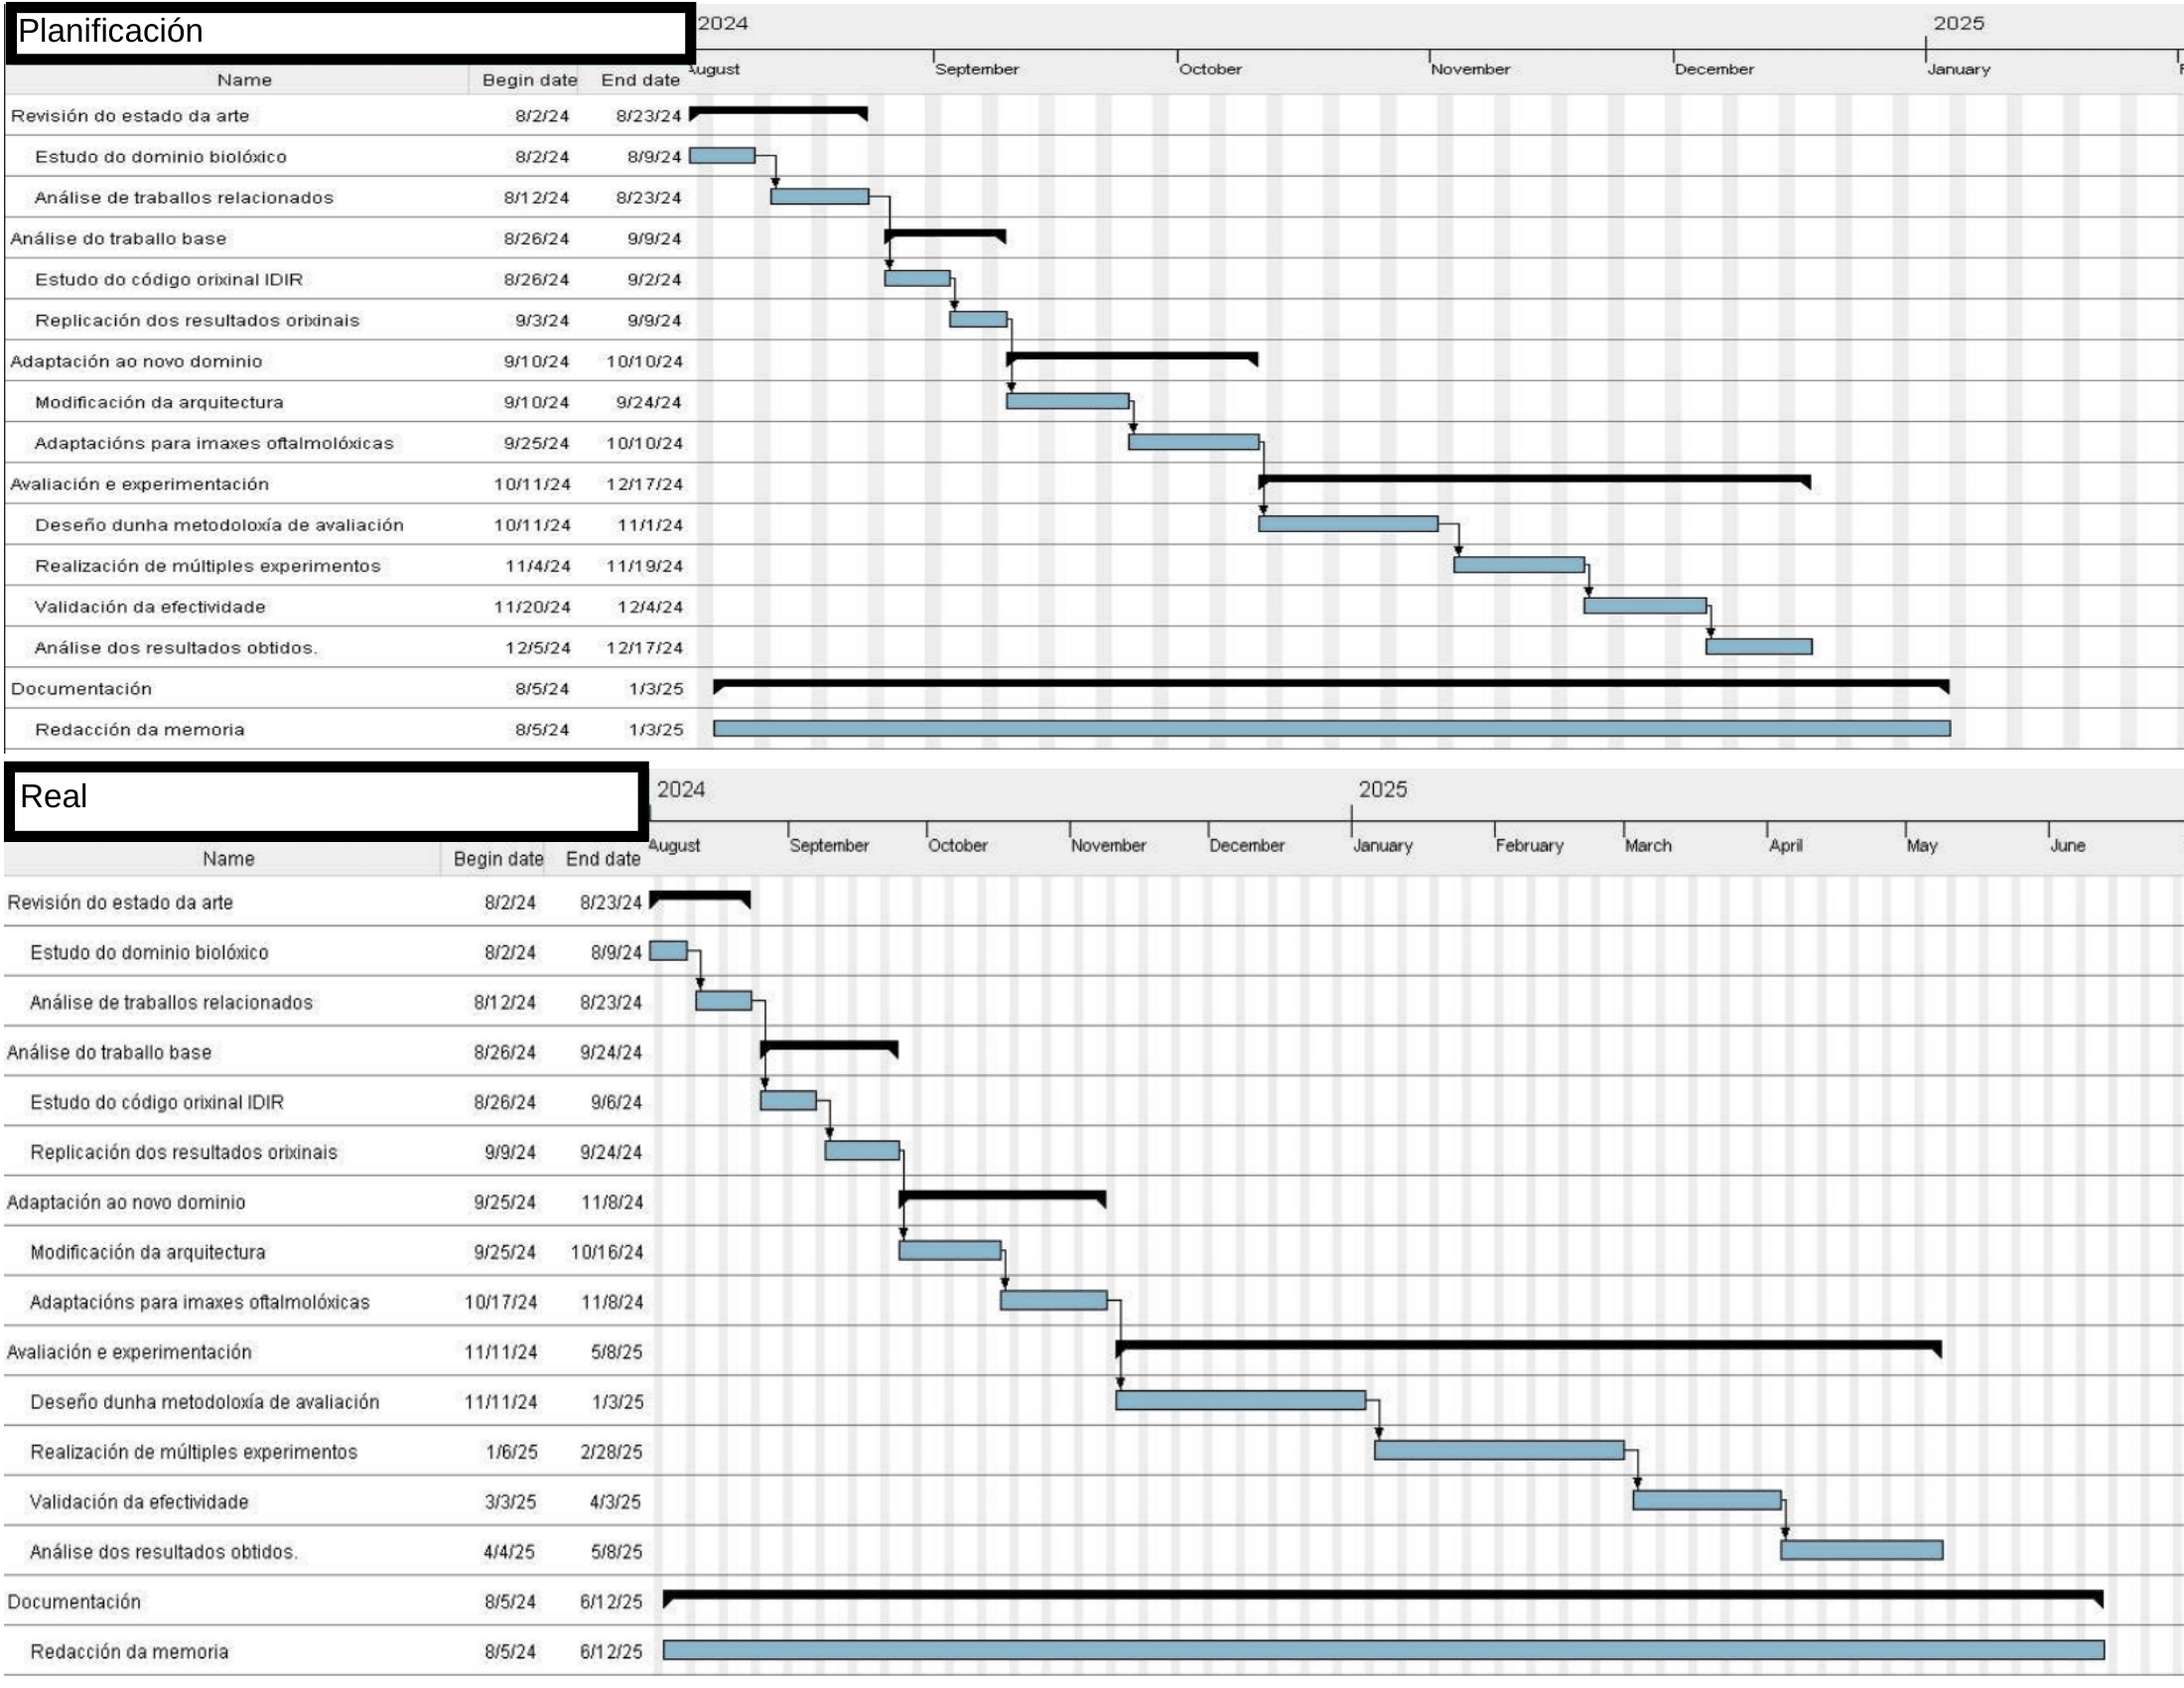
\includegraphics[height=1\textwidth, angle=90]{imaxes/gants-1.png}
    \caption{Gantt diagrams of project planning and actual duration of each phase}
    \label{fig:planificacion_proxecto}
\end{figure}

\section{Resources Used}
\label{sec:Recursos utilizados}

\subsection{Software}
\label{subsec:Software}

Since part of the work consists of adapting previous work, 
it was decided to use much of the same software as the original work to facilitate implementation and reproducibility.
The most relevant is PyTorch, an open-source library for Python that facilitates the development of neural networks. Python 3.12.3 and CUDA 12.2 versions were used. Support libraries such as NumPy (for working with matrices), Matplotlib (visualization), OpenCV, or scikit-learn (image handling) are also used.

Other software used includes VSCode (IDE), Git (version control), and LaTeX (report writing).

\subsection{Hardware}
\label{subsec:Hardware}

The project was developed on a laptop connected via ssh to a server with GPU. 
Two different servers were used, one set up by me\footnote{\url{https://blog.m19182.dev/writings/Building-my-Homelab}} and another provided by the VARPA research group (Artificial Vision and Pattern Recognition).

Most experiments were conducted on the first one, but to run the project with images at their original resolution, it was necessary to use the second one
due to GPU memory limitations. Table \ref{tab:comparativa_servidores} shows a comparison between the servers used, indicating the main hardware characteristics of each.

\begin{table}[tbp]
\centering
\begin{tabular}{|c|c|c|}
\hline
\textbf{Characteristic} & \textbf{Personal Server} & \textbf{VARPA Server} \\ \hline
Processor & AMD Ryzen 9 5950X&  AMD Ryzen Threadripper 3960X \\ \hline
GPU & NVIDIA RTX 3090 & NVIDIA RTX A6000  \\ \hline
\end{tabular}
\caption{Comparison between the servers used}
\label{tab:comparativa_servidores}
\end{table}


\subsection{Datasets}
\label{subsec:Conxuntos de datos}
Two different datasets were used for the project development:

\begin{itemize}
    \item \textbf{RFMID:} 3200 color fundus images with 1712x1712 resolution.
    \item \textbf{FIRE:} 134 pairs of color retinal images, with a size of 2912×2912 pixels
\end{itemize}

These are described in more detail in section \ref{sec:Conxuntos de datos}.

\subsection{Cost Estimation}
\label{subsec:Estimación de custos}

Hardware costs are ignored as they were already available before the project began.

Human resource costs are calculated for one student and two tutors, resulting in an estimated cost of €20,680, VAT included. Table \ref{tab:estimacion_custos} shows the breakdown of estimated human resource costs, considering a student at €20/hour and tutors at €35/hour.

\begin{table}[h]
\centering
\begin{tabular}{|c|c|c|c|}
\hline
\textbf{Resource} & \textbf{Cost per hour} & \textbf{Estimated hours} & \textbf{Total cost} \\ \hline
Student & €20 & 880h & €17,600 \\ \hline
Tutor 1 & €35 & 44h & €1,540 \\ \hline
Tutor 2 & €35 & 44h & €1,540 \\ \hline
\end{tabular}
\caption{Estimation of human resource costs (VAT included)}
\label{tab:estimacion_custos}
\end{table}

\section{Planning Follow-up}
\label{sec:Seguimento da planificación}

The project planning was periodically reviewed according to project phases, and to identify deviations from the initial plan.

Although the initial phases of the project adhered to the planning, the adaptation to new domain phase and the evaluation and experimentation phase experienced significant delays.

The adaptation to new domain phase required more time than expected due to the complexity of modifications needed to adapt the model to 2D images, as well as the need to perform multiple tests to ensure proper functioning of the adapted model. The evaluation phase was also affected, as it required more time than expected to design an appropriate evaluation methodology. Finally, the experimentation phase required more time than anticipated, partly due to poor initial results, which required an in-depth code review and implementation of new tests to ensure correct implementation.
In total, this led to a delay of approximately 18 weeks from the initial planning.

The final phase of results analysis and report writing was also affected, although to a lesser extent, which led to an additional 2-week delay, resulting in a total project duration of 40 weeks, compared to the initially planned 20 weeks.

Figure \ref{fig:planificacion_proxecto} shows the updated Gantt chart, reflecting the actual duration of each project phase.

\subsection{Actual Cost Estimation}
\label{subsec:Estimación de custo real}

The project cost estimation was €20,680, as indicated in section \ref{subsec:Estimación de custos}. However, due to delays in project development, the actual cost increased proportionally to the extra time spent.

Since the project extended for 20 more weeks than planned (double the initial planning), the estimated actual cost amounts to €41,360 (VAT included).